
\documentclass[a4paper,12pt]{article}
\usepackage[margin=22mm]{geometry}
\usepackage{fontspec,xltxtra,polyglossia,titling,graphicx}
\usepackage{caption}  \captionsetup[table]{skip=6pt}
\usepackage{verbatim,synttree,multicol,booktabs,gb4e}
\noautomath
\usepackage[colorlinks,urlcolor=blue,citecolor=blue,linkcolor=blue]{hyperref}
\setmainfont[Mapping=tex-text]{Times New Roman} % or another similar font
\usepackage[backend=biber, style=authoryear, citestyle=authoryear-comp, maxcitenames=2, maxbibnames=50, language=auto, isbn=false, doi=true]{biblatex} % may produce a warning
\frenchspacing


\title{Assignment-03} % replace with title of your term paper
\author{MS18006} % replace with your candidate number, not your name
\newcommand{\Coursecode}{Extreme Weather} % replace with course code and name
\newcommand{\Semester}{April 12 2023}

\setdefaultlanguage{english} % endre til norsk om du vil
\setotherlanguages{norsk}

\addbibresource{sample.bib}

\newcommand{\tig}[1] {\fontspec{Abyssinica SIL} #1} % example fontspec for Tigrinya

\hyphenation{lem-mat-iz-at-ion uni-code}

\begin{document}
\begin{center} \vfill
\thispagestyle{empty}
\textbf{\Large Indian Institute of Science Education and Research (IISER), Mohali}

{\large EES405 Climate Data Analysis and Visualisation

\Coursecode

\Semester} \vfill


\includegraphics[width=70mm]{pics/HighResolutionLogo.jpg} \vfill

\emph{\Large \thetitle} \vfill

{\large \theauthor} \vfill

\end{center} \clearpage
 \maketitle

% \begin{abstract} \noindent
% This template is provided for papers at the bachelor's and master's programs in Linguistics at the University of Bergen, Norway.
% It demonstrates the use of \LaTeX, a document preparation system which is quite suited to scientific papers and theses.
% This document is not intended to give a realistic example of linguistic content, but attempts to demonstrate many different textual elements that are common in a term paper or a bachelor's thesis.
% \end{abstract}



% Examples, figures, tables, equations and appendices should always be numbered.
% This is done automatically.
% The use of labels and references to those labels ensures that the correct numbers are produced.

% Linguistic examples should be provided with translations if they are not in the language of the paper.
% If the morphological structure of words is relevant for the discussion, or helpful for the reader in order to understand the sentence, please use interlinear glosses according to the Leipzig Glossing Rules.\footnote{Leipzig Glossing Rules: \url{https://www.eva.mpg.de/lingua/resources/glossing-rules.php}}

% Examples (\ref{ex:dutch}) and (\ref{ex:tigrinya}) illustrate the inclusion of interlinear glosses and translations.
% Example (\ref{ex:tigrinya}) also illustrates the use of a specific font for the Ge‛ez script which is used to write the Ethiopian and Tigrinya alphabets. 

% \begin{exe}
% \ex \label{ex:dutch}
% \gll Dit is een Nederlands voorbeeld-je.\\
% This is a Dutch example-DIM\\
% \trans `This is a small example in Dutch.'

% \ex \label{ex:tigrinya}
% \glll \tig{መይቱዋ/ላ።}\\
% mäyit-u-wa/la\\
% PerfS.die-SM.3MSg-OM$_1$/OM$_2$.3MSg\\ % use math mode for subscript
% \trans ‘He died on/for her.’
% \end{exe}

% Also equations and formulas are numbered, as shown in Equation \ref{eq:lix}.
% Figure \ref{fig:tree} illustrates how a tree structure can be drawn from a labeled bracketing representation.

% \begin{equation} \label{eq:lix}
% Lix=\frac{W}{S}+\frac{L \cdot 100}{W}
% \end{equation}

% \begin{figure}[htbp] \begin{center}
% \synttree [S [NP [Pro [He]]] [VP [V [died]] [PP [P [for]] [NP [Pro [her]]]]]]
% \caption{An example tree drawn from labeled bracketing using the \emph{synttree} package.} \label{fig:tree}
% \end{center} \end{figure}

% \section{Data and Method}
% It is often appropriate to devote a section to the description of the data and method.
% This section could, for instance, describe corpus materials, lexical data, questionnaires, experimental procedures, annotation software or other data, methods and tools which you have used for your paper.
% Be specific in your description and specify where each resource was obtained.
% If you search in a corpus, for instance, specify which corpus was consulted on which site, and give your exact search expressions.

% Provide datasets, sample questionnaires, lists of experimental stimuli or other materials in numbered appendices.
% However, materials spanning more than a page should preferably not be included in the PDF, but can be bundled in a ZIP or RAR archive together with the main file.
% Alternatively, large files can be uploaded on one of the university's platforms, such as OneDrive or GitLab.

% \section{Results}
% This section could describe the results obtained from the research.
% Present quantitative results in tables, plots and diagrams, as illustrated in Table \ref{tab:pct} and in Figures \ref{fig:bp} and \ref{fig:cm}.
% It is highly advisable to produce the text and commands for tables directly from analysis scripts.
% Python as well as R can produce good \LaTeX\ code for tables.
% Plots and other graphs can be exported to files by analysis scripts and included for typesetting.
% This is usually preferable to making screenshots.
% Make sure that text in your tables and figures is easily readable.

% \begin{table}
\centering
\caption{Caption at the top of a table.}
\label{tab:pct}
\begin{tabular}{lrr}
\toprule
{} &     f &     m \\
Word     &       &       \\
\midrule
beat     &  31.7 &  68.3 \\
bloke    &  36.0 &  64.0 \\
cat      &  65.4 &  34.6 \\
clothes  &  69.1 &  30.9 \\
cool     &  30.3 &  69.7 \\
crap     &  35.5 &  64.5 \\
football &  24.1 &  75.9 \\
kiss     &  81.5 &  18.5 \\
love     &  72.2 &  27.8 \\
model    &  88.2 &  11.8 \\
music    &  45.8 &  54.2 \\
phone    &  70.9 &  29.1 \\
\bottomrule
\end{tabular}
\end{table}

% \begin{figure}[htbp] \begin{center}
% \includegraphics[width=0.7\textwidth]{boysgirls.png}
% \caption{Caption of a bar plot} \label{fig:bp}
% \end{center} \end{figure}

% \begin{figure}[htbp] \begin{center}
% 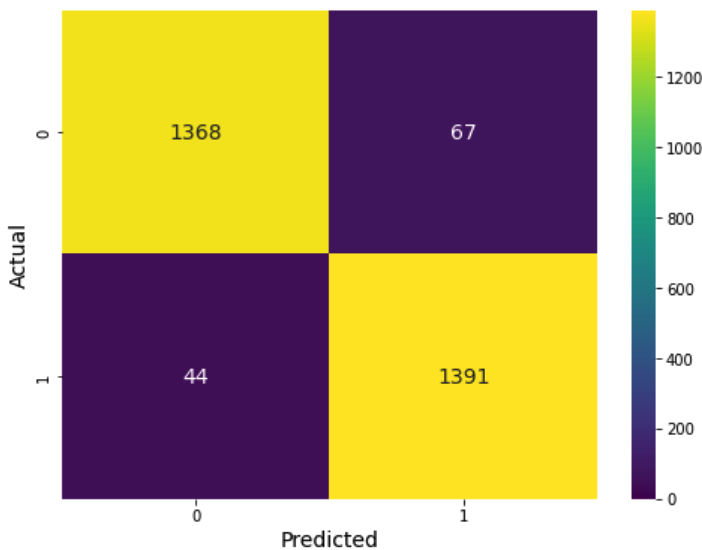
\includegraphics[width=0.6\textwidth]{cm.png}
% \caption{Caption of a heatmap} \label{fig:cm}
% \end{center} \end{figure}

% \section{Discussion and conclusion}
% The last section is an opportunity to interpret the results and to assess if the results confirm or reject the initial hypothesis formulated in section \ref{sec:intro}.
% The conclusion summarizes which new knowledge is obtained, and possibly what it can be used for.
% If relevant, a comparison can be made with other studies.
% It also discusses to what extent the outcomes are uncertain or of a limited scope.

% Include relevant references to related work \parencite{Kopka04,Mittelbach04,Van_Dongen12}.
% This is achieved with cite commands which automatically take references from a list of publications (your .bib file) and adds them to the bibliography at the end of the document.
% Such automatic management of references ensures a consistent chosen style.
% The best way to manage a bibliography file is through a dedicated reference manager, such as Zotero\footnote{Zotero: \url{https://www.uib.no/en/ub/143203/zotero}, \url{https://zotero.org}} or BibDesk.
% You can export items from Zotero to a bibfile that you upload to Overleaf.
% Remember to pin the bibkeys before export from Zotero, because those are used in the citation commands.

% There are several styles for the bibliography; the one used in this example is \emph{author-date}.\footnote{Here is a compact guide to BibLaTeX: \url{http://tug.ctan.org/info/biblatex-cheatsheet/biblatex-cheatsheet.pdf}} 
% References to web resources can also be put in footnotes.\footnote{Wikibooks: \url{https://en.wikibooks.org/wiki/LaTeX}} 

% Quotations from other works should either be marked in the text with quotation marks, or should be in separate paragraphs marked with indentation, and should always be provided with a citation of the source.
% Translate if appropriate, as in the following.

% \begin{quote}
%     It is up to the psychologist to determine the exact place of semiology; the task of the linguist is to define what makes language [\textit{langue}] a special system within the whole of the semiological facts. \parencite[p. 33; my translation]{Saussure16}
% \end{quote}

% \LaTeX\ takes a while to learn, but it pays off in the long run because so much can be automated and made consistent.
% You might be overwhelmed by the many different things in this brief template, but don't be scared: just use what you need and leave the rest for later.

% \printbibliography

% \clearpage
% \appendix
% \section{Frequency list >= 5} \label{app:freq}
% This is an example appendix showing how small amounts of data or results  can be included literally from a separate file and written over multiple columns.

% \begin{multicols}{3}
% % Use \verbatiminput to input literal plain text from files
% {\footnotesize\verbatiminput{askefreqnohapax}}
% \end{multicols}

\section{Problem 1 } \label{sec:q1}
\subsection{Spatial distribution of Rainfall over India ONLY}






\end{document}